\subsection{Q15 Format} \label{sec:q15}

For our filter design, fixed format number format called Q is used. Unlike floating point numbers, Q-format numbers require only standard integer ALU to perform rational number calculations. This means that we do not need to add an FPU to our design which requires additional power.

Q format numbers are represented using the Q notation which is written as Q$m,n$ where $m$ is the number of bits set aside to designate the two's complement integer portion of the number, and $n$ is the number of bits used to designate the fractional portion of the number.

In our case, we use simplified notation Q$n$ since we assume that the numbers are normalized into the range of $[-1, 1)$. Notice that this assumption does not affect the generality of the filter, but it simplifies the multiplication operation because the multiplication result never exceeds the range of $[-1, 1)$.

\begin{figure}[ht]
	\centering
	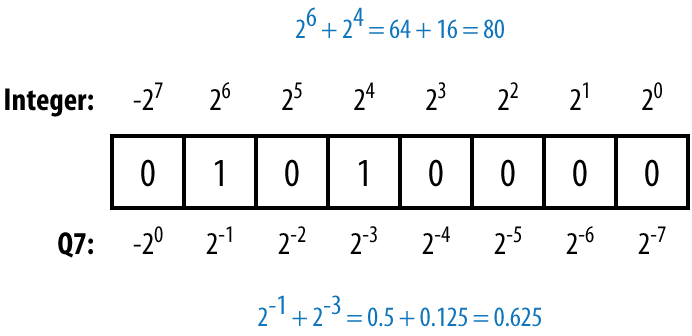
\includegraphics[scale=1.5]{images/q7}
	\caption{Comparison between integer and Q7 format.}
	\label{fig:q7}
\end{figure}

Figure \ref{fig:q7} shows the comparison between two's complement integer and Q7 numbers. The only difference between the two is the weight assigned for each bit.

\subsection{Filter Characteristics}

The coefficients for the filter is shown in Table \ref{tab:coefficients}. These values were computed using Filter Design \& Analysis Tool in Matlab Signal Processing Toolbox which is one of the most widely used filter design tool in the industry. 

\begin{table}[ht]
\centering
\begin{tabular}{ c | r }
\hline
Coeffiecient & Value \\
\hline \hline
$C_0$ & -1.55107884796477e-18 \\
$C_1$ & -0.022663985459552 \\
$C_2$ & 1.04697822237622e-17 \\
$C_3$ & 0.273977082565524 \\
$C_4$ & 0.497373805788057 \\
$C_5$ & 0.273977082565524 \\
$C_6$ & 1.04697822237622e-17 \\
$C_7$ & -0.0226639854595526 \\
$C_8$ & -1.55107884796477e-18 \\
\end{tabular}
\caption{Coefficient values}
\label{tab:coefficients}
\end{table}


\begin{figure}[ht]
	\centering
	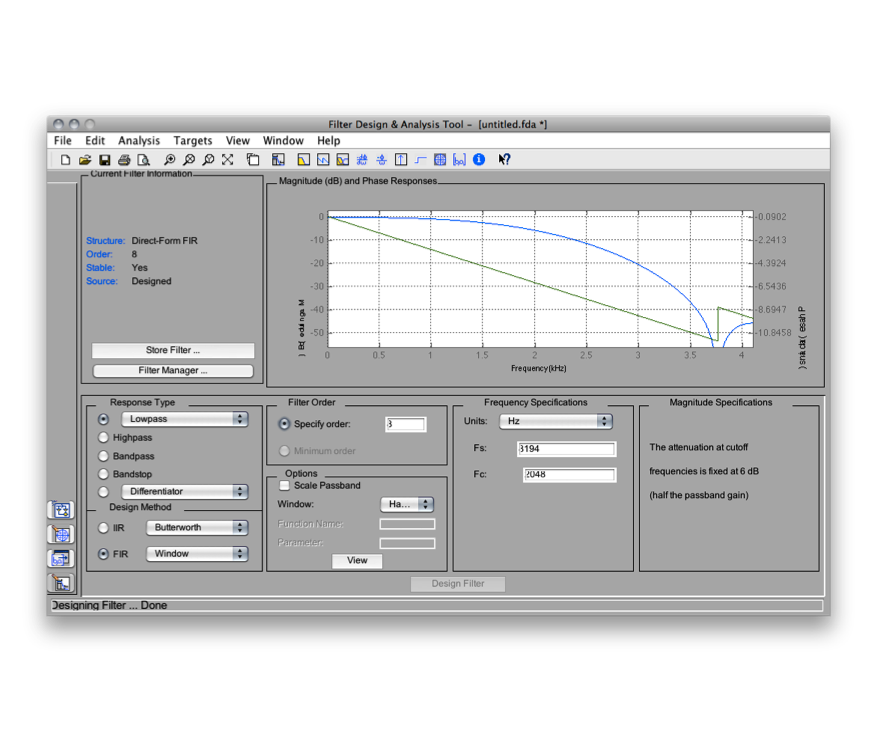
\includegraphics[scale=1]{images/matlab}
	\caption{Matlab Filter Design \& Analysis Tool.}
	\label{fig:matlab}
\end{figure}
